\documentclass[journal]{IEEEtran}

\usepackage{amsmath,amssymb,amsfonts,amsthm}
\usepackage{graphicx}
\usepackage{booktabs}
\usepackage{multirow}
\usepackage{cite}
\usepackage{xcolor}
\usepackage{placeins}
\usepackage{hyperref}

\hypersetup{colorlinks=true,linkcolor=blue,citecolor=blue,urlcolor=blue}
\graphicspath{{../../figures/}}
\renewcommand{\arraystretch}{1.12}
\newtheorem{proposition}{Proposition}
\newtheorem{corollary}{Corollary}

\begin{document}

\title{When Do Amplitude-Encoding Quantum Kernels Help Security Anomaly Detection? A Matched-Scale Study on QKD Telemetry and Network Intrusion Data}

\author{Arnav~Kapoor%
\thanks{A. Kapoor is with the Department of Computer Science, Indian Institute of Science Education and Research Bhopal, Bhopal 462066, India (e-mail: arnavkapoor23@iiserb.ac.in).}}

\markboth{Manuscript}{Kapoor: Amplitude-Encoding Kernels for Security Anomaly Detection}

\maketitle

\begin{abstract}
Amplitude encoding is the most common way of loading classical data into
quantum kernels proposed for security tasks. Its fidelity kernel is exactly the
squared cosine similarity of the inputs, so it can be evaluated at any scale and
compared fairly with classical kernels. We do so on four datasets in two
domains---QKD physical-layer telemetry from a decoy-state BB84 simulator with
operating drift, and zero-trust network flows from a controlled simulator,
UNSW-NB15 and CIC-IDS2017---training every model on the same data at every
training size. In distribution, the amplitude-encoding SVM is never better than
an RBF-kernel SVM (e.g.\ $0.862$ vs.\ $0.863$ accuracy on UNSW-NB15), needs more
data at small $n$, and trails tree ensembles and neural networks. On attack types
withheld from training the picture is domain-dependent. In both controlled
settings where unseen attacks differ from normal traffic mainly in magnitude, it
fails (mean held-out AUC $0.53$ vs.\ $0.84$ for RBF on synthetic flows; $0.55$ vs.\
$0.94$ on QKD telemetry without its one magnitude-carrying feature); a
norm-anchored encoding that appends one constant coordinate repairs this ($0.79$,
$0.94$), and interventions confirm the kernel's norm invariance as the cause. On
the two public benchmarks it does not fail: it matches or slightly exceeds RBF
(@ZD_ABS_MERGED@), though both kernels trail tree ensembles and a benign-only
autoencoder on CIC-IDS2017. A simple norm-separability statistic does not predict
which case a dataset falls into, so we recommend testing unseen-attack
generalization directly. We also find that a Gaussian-process posterior is a
worse basis for alert deferral than an isotonic-calibrated random forest, and
that drift-free QKD simulators are trivially separable. Code, data preparation
and all result files are released.
\end{abstract}

\begin{IEEEkeywords}
Quantum machine learning, quantum kernels, amplitude encoding, intrusion detection, quantum key distribution, zero-day attacks, calibration, negative results.
\end{IEEEkeywords}

\section{Introduction}
\label{sec:intro}

\IEEEPARstart{Q}{uantum} kernel methods map data into the Hilbert space of a
quantum register and use state overlaps as a kernel~\cite{havlicek2019supervised,schuld2021machine}.
They are increasingly proposed for security tasks, from intrusion
detection~\cite{kalinin2023security} to botnet traffic
classification~\cite{suryotrisongko2022evaluating}, usually on the strength of
their novelty and of encouraging accuracy at a single operating point. Two
facts make such results hard to interpret. First, whether a quantum kernel helps
depends on how its geometry matches the data~\cite{huang2021power}; provable
advantages exist only for specially constructed problems~\cite{liu2021rigorous}.
Second, quantum kernels are often trained on far fewer samples than the
classical baselines they are compared with, because circuit simulation is slow,
so model and data size are confounded.

This paper studies the most common encoding in this literature, amplitude
encoding, whose fidelity kernel is exactly the squared cosine similarity of the
inputs (Proposition~\ref{prop:exact}). Because it is classically computable, we
can evaluate it at any scale, against classical kernels trained on identical
data, and ask a question that does not depend on quantum hardware: \emph{is its
inductive bias useful for security anomaly detection, and if so when?}

We answer it in two structurally different domains. The first is
physical-layer telemetry from quantum key distribution (QKD) links, where
implementation attacks such as photon-number splitting~\cite{huttner1995photon},
detector blinding~\cite{lydersen2010hacking}, Trojan-horse
probing~\cite{gisin2006trojan} and intercept-resend~\cite{bennett1992experimental}
perturb channel statistics. The second is network-flow monitoring for zero-trust
architectures~\cite{rose2020zero,syed2022zero}, evaluated on a controlled flow
simulator and on two public benchmarks, UNSW-NB15~\cite{moustafa2015unsw} and
CIC-IDS2017~\cite{sharafaldin2018toward}.

\textbf{Contributions.}
\begin{enumerate}
\item \textbf{A matched-scale comparison} of the amplitude-encoding kernel with
  RBF, Laplacian and polynomial kernels, tree ensembles and neural networks, all
  trained on identical data at every training size, across four datasets in two
  security domains (Section~\ref{sec:res-indist}--\ref{sec:res-matched}).
\item \textbf{A domain-dependent zero-day effect, its mechanism and a fix.}
  The kernel fails on unseen attack types in two controlled settings and not on
  two public benchmarks. Interventions---removing a magnitude-carrying feature,
  removing sign ambiguity, and a one-coordinate norm anchor---identify norm
  invariance as the cause where it fails (Sections~\ref{sec:kernel},
  \ref{sec:res-zeroday}, \ref{sec:res-mechanism}).
\item \textbf{Evidence on uncertainty for alert deferral:} a Gaussian-process
  posterior is less calibrated, and supports a worse coverage--accuracy
  trade-off, than an isotonic-calibrated random forest (Section~\ref{sec:res-calib}).
\item \textbf{A QKD telemetry simulator with leakage tests} and an attack-strength
  axis, motivated by our finding that a drift-free simulator is trivially
  separable (Section~\ref{sec:qkd-data}).
\end{enumerate}

Section~\ref{sec:background} reviews related work. Section~\ref{sec:kernel}
analyses the kernel. Section~\ref{sec:protocol} gives the evaluation protocol,
Section~\ref{sec:data} the four datasets, and Section~\ref{sec:results} the
results. Section~\ref{sec:discussion} discusses implications and threats to
validity.

\section{Background and Related Work}
\label{sec:background}

\subsection{Quantum and quantum-inspired kernels}
A quantum kernel evaluates $k(\mathbf{x},\mathbf{y})=|\langle\psi(\mathbf{x})|\psi(\mathbf{y})\rangle|^2$
for a data-dependent state $|\psi(\cdot)\rangle$~\cite{havlicek2019supervised}.
For entangling feature maps the kernel can be classically hard to evaluate, and
Liu et al.~\cite{liu2021rigorous} prove an end-to-end speed-up for a problem built
on the discrete logarithm. Huang et al.~\cite{huang2021power} show that even
classically hard kernels need not beat classical learners on real data, and
give a geometric test for when they can. Amplitude encoding, which loads a
normalized vector into the amplitudes of $\lceil\log_2 d\rceil$ qubits, is the
opposite case: its kernel is classically easy, so any benefit it has must come
from its inductive bias. Classical random-feature approximations~\cite{rahimi2007random}
and Nystr\"om methods~\cite{williams2001nystrom} make any such kernel usable at scale.
Adversarial vulnerability of quantum classifiers is studied by Lu et
al.~\cite{lu2020quantum}.

\subsection{Machine learning for QKD attack detection}
Countermeasures to implementation attacks include hardware monitoring of
detector statistics~\cite{dasilva2012monitoring} and protocol changes such as
decoy states~\cite{lo2005decoy} and measurement-device-independent
QKD~\cite{lo2012measurement}. Mao et al.~\cite{mao2020detecting} use neural
networks to recognise attacks on continuous-variable QKD; Ren et
al.~\cite{ren2021machine} use machine learning for protocol and parameter
selection. Such studies are almost always run on simulated telemetry, which
raises the question of whether a simulator is hard enough to discriminate
between methods (Section~\ref{sec:qkd-data}).

\subsection{Network intrusion detection}
Machine-learning intrusion detection is surveyed by Buczak and
Guven~\cite{buczak2016survey}; Sommer and Paxson~\cite{sommer2010outside}
caution that detectors which perform well on a closed set of attacks often fail
on new ones, which is why we evaluate generalization to unseen attack families
directly. Kitsune~\cite{mirsky2018kitsune} popularised unsupervised autoencoder
detectors, which never see attack labels and so form a natural zero-day
reference. Zero-trust architectures~\cite{kindervag2010build,rose2020zero,gilman2017zero}
make continuous flow-level monitoring part of the access decision.

\subsection{Calibration and certified robustness}
Security operators act on alert confidence, so probability calibration
matters~\cite{guo2017calibration}. Gaussian processes~\cite{rasmussen2006gaussian}
and other Bayesian models~\cite{perusquia2022bayesian} provide model-based
uncertainty; Platt scaling~\cite{platt1999probabilistic} and isotonic
regression~\cite{zadrozny2002transforming} recalibrate point estimators.
Randomized smoothing~\cite{cohen2019certified} certifies $\ell_2$ robustness for
any base classifier.

\section{The Amplitude-Encoding Kernel}
\label{sec:kernel}

For $\mathbf{x}\in\mathbb{R}^d$, amplitude encoding zero-pads $\mathbf{x}$ to
$2^q$ entries, $q=\lceil\log_2 d\rceil$, normalizes it, and prepares
$|\psi(\mathbf{x})\rangle=\sum_i \hat{x}_i|i\rangle$ with
$\hat{\mathbf{x}}=\mathbf{x}/\|\mathbf{x}\|_2$.

\begin{proposition}[Exact classical form]\label{prop:exact}
The fidelity kernel of amplitude encoding is
\begin{equation}
K_A(\mathbf{x},\mathbf{y}) = |\langle\psi(\mathbf{x})|\psi(\mathbf{y})\rangle|^2
= \frac{(\mathbf{x}^{\mathsf{T}}\mathbf{y})^2}{\|\mathbf{x}\|_2^2\,\|\mathbf{y}\|_2^2},
\label{eq:ka}
\end{equation}
computable in $\mathcal{O}(d)$ time per pair.
\end{proposition}
\begin{proof}
The amplitudes are real and the padding entries are zero, so
$\langle\psi(\mathbf{x})|\psi(\mathbf{y})\rangle=\hat{\mathbf{x}}^{\mathsf{T}}\hat{\mathbf{y}}$.
\end{proof}

$K_A$ is the homogeneous degree-2 polynomial kernel applied to normalized
inputs, so its feature space is spanned by the products $\hat{x}_i\hat{x}_j$.
Two invariances follow directly and drive the results below.

\begin{corollary}[Norm and sign invariance]\label{cor:inv}
$K_A(c\,\mathbf{x},\mathbf{y})=K_A(\mathbf{x},\mathbf{y})$ for every $c\neq0$. Any
classifier built on $K_A$ assigns the same score to $\mathbf{x}$, $2\mathbf{x}$ and
$-\mathbf{x}$; it cannot use the distance of an input from the origin.
\end{corollary}

On standardized features the origin is the mean of the training data, so the
distance from the origin is exactly the quantity an outlier detector would
use. Corollary~\ref{cor:inv} therefore predicts that $K_A$ helps when labels
depend on direction and the norm is a nuisance, and hurts when an attack is
recognisable mainly by being \emph{far} from normal traffic, which is the
typical situation for an attack never seen in training.

\textbf{Norm anchoring.} A standard way to retain the norm is to append a
constant coordinate before encoding:
\begin{equation}
\phi_c(\mathbf{x}) = \frac{(\mathbf{x},\,c)}{\sqrt{\|\mathbf{x}\|_2^2+c^2}},
\qquad c=\operatorname{median}_{\mathbf{x}\in\mathcal{D}_{\mathrm{train}}}\|\mathbf{x}\|_2 .
\label{eq:anchor}
\end{equation}
The last amplitude, $c/\sqrt{\|\mathbf{x}\|^2+c^2}$, is a monotone function of
$\|\mathbf{x}\|$, and the sign of $\mathbf{x}$ is no longer ambiguous. The
median-norm rule fixes $c$ from training data alone. The encoding needs one
extra amplitude (at most one extra qubit).

\textbf{Sensitivity.} The Jacobian of $\mathbf{x}\mapsto\hat{\mathbf{x}}$ is
$(I-\hat{\mathbf{x}}\hat{\mathbf{x}}^{\mathsf{T}})/\|\mathbf{x}\|_2$, with spectral norm
exactly $1/\|\mathbf{x}\|_2$. Normalization contracts perturbations of large-norm
inputs but amplifies those of inputs near the origin, so it provides no uniform
robustness guarantee; this matches the certified-robustness results in
Section~\ref{sec:results}.

\textbf{Implementation check.} We evaluate Eq.~\eqref{eq:ka} in closed form and
verify it against a PennyLane~\cite{bergholm2018pennylane} state-vector
simulation of the overlap circuit $\langle0|U^\dagger(\mathbf{y})U(\mathbf{x})|0\rangle$.
The two agree to $7\times10^{-15}$; the simulated circuit takes $26$\,ms per kernel
entry against $3\times10^{-4}$\,ms in closed form, a factor of about $8\times10^{4}$.
Training-set limits of a few dozen samples that are sometimes attributed to
quantum kernels are therefore a property of circuit simulation, not of this
kernel.

\section{Evaluation Protocol}
\label{sec:protocol}

\textbf{Matched scale.} Every model in a comparison is trained on the same
training subsample, at every training size $n$ we report; feature
dimensionality is matched the same way. Confidence intervals are 95\% intervals
over seeds (10 for the QKD and synthetic-flow benchmarks, 5 for the public
datasets, 3 for leave-one-family-out runs on public data).

\textbf{Models.} AE-SVM uses $K_A$; AE-SVM (anchored) uses $K_A\circ\phi_c$. The
classical kernels are RBF ($\gamma=1/(d\,\mathrm{Var}[\mathbf{x}])$), Laplacian and
cubic polynomial, all in the same SVM. Exact kernel SVMs are used up to
$1{,}500$ training samples and a Nystr\"om approximation~\cite{williams2001nystrom}
with $m$ uniformly sampled landmarks above that ($m=\lceil0.1n\rceil\le500$ on
synthetic flows, $m=1000$ on public data); RBF, Laplacian and polynomial kernels
use the same wrapper. Other baselines are random forests (RF, 200
trees)~\cite{breiman2001random}, XGBoost~\cite{chen2016xgboost}, a two-layer MLP,
and, on public data, a $3\times256$ deep network (DNN) with batch normalization,
dropout and early stopping, and a Kitsune-style autoencoder~\cite{mirsky2018kitsune}
trained on benign traffic only. On QKD telemetry we also include a Laplace
Gaussian-process classifier (GP)~\cite{rasmussen2006gaussian}, a GP+AE-SVM
stacking model~\cite{wolpert1992stacked}, isotonic-calibrated RF, and three
novelty detectors fit on normal data (one-class SVM, isolation forest, LOF).

\textbf{Measurements.} In-distribution detection (accuracy, F1, MCC, ROC-AUC);
learning curves at matched $n$; leave-one-attack-out generalization, training on
all but one attack type or family and testing on benign traffic plus the
held-out one (ROC-AUC, which does not depend on a threshold tuned to known
attacks); kernel-target alignment~\cite{cristianini2002kernel}; expected
calibration error (ECE, 15 bins) and selective prediction; randomized-smoothing
certified radii~\cite{cohen2019certified}; and inference latency with training
excluded. Paired comparisons use paired $t$-tests over seeds or exact McNemar
tests on test predictions.

\section{Datasets}
\label{sec:data}

\subsection{QKD telemetry}
\label{sec:qkd-data}
Each sample is one key-generation block of a decoy-state BB84 link over 50\,km of
fiber, with Poisson-source gain and QBER~\cite{lo2005decoy}. Normal operation
includes per-block drift in attenuation, detector efficiency, misalignment,
dark counts and background light, and finite-size noise on the two estimated
error rates. Seven measurements are reported per block. Four attacks perturb
them; every perturbation is scaled by a strength $s$, so $s=1$ is the default
signature and $s\to0$ makes an attack indistinguishable from normal operation.
Features are the 7 measurements, standardized, plus a robust Mahalanobis
distance~\cite{rousseeuw1999fast} to training-split normal blocks; the
Mahalanobis coordinate turns out to matter (Section~\ref{sec:res-zeroday}). We
report $s=1$ and the harder $s=0.3$; $N=2000$ blocks with 30\% attacks.

Without drift this kind of simulator is trivially separable: in our own first
version, a single feature (the error rate) separated attacks perfectly, and
every model scored near $1.0$. We therefore release leakage tests (independent
seeds; no single-feature label proxy) with the simulator.

\subsection{Synthetic zero-trust flows}
Flow records are $d$-dimensional feature vectors (default $d=64$: 16
header, 24 flow and 24 behavioral features) whose marginals follow commonly
reported NetFlow statistics (Pareto packet rates, log-normal byte rates, Weibull
durations) and are coupled by a Gaussian copula with within-group correlation
$0.35$. Five attacks (port scan, DDoS, exfiltration, DNS tunneling, ARP spoofing)
shift and inflate the variance of 6--7 attack-specific latent dimensions by
$1.4$--$2.6\sigma$. $N=8000$ flows with 20\% attacks; features are standardized.

\subsection{Public benchmarks}
\textbf{UNSW-NB15}~\cite{moustafa2015unsw}: the official partition (175,341
training and 82,332 test records) with 39 numeric features and one-hot
protocol, service and state (68 features); nine attack families. Its test
partition is known to be distributionally shifted from its training partition.
\textbf{CIC-IDS2017}~\cite{sharafaldin2018toward}: the eight MachineLearningCVE
day files (2,830,743 flows). We drop rows with missing or infinite values,
remove 308,381 exact duplicates and constant columns (69 features remain), drop
classes with fewer than 100 flows, group labels into six families (DoS, DDoS,
PortScan, BruteForce, WebAttack, Bot) and use a fixed stratified 70/30 split.
Both: features are mapped through $\operatorname{sign}(x)\log(1+|x|)$, and each seed
draws a family-stratified training subsample of 20,000 flows and a test
subsample of 50,000 flows.

\section{Results}
\label{sec:results}

\subsection{In-distribution detection}
\label{sec:res-indist}

\begin{table*}[t]
  \centering
  \caption{In-distribution detection (mean $\pm$ 95\% CI over seeds). QKD: MCC and AUC at attack strength $s=0.3$, $n=1400$, 10 seeds. Synthetic flows: accuracy and AUC, $n=5600$, 10 seeds. Public data: F1 and AUC on 50,000 test flows, $n=20{,}000$, 5 seeds. -- = not run in that domain.}
  \label{tab:indist}
  \scriptsize
  \setlength{\tabcolsep}{3.2pt}
  \begin{tabular}{lcccccccc}
    \toprule
    & \multicolumn{2}{c}{QKD telemetry ($s{=}0.3$)} & \multicolumn{2}{c}{Synthetic flows} & \multicolumn{2}{c}{UNSW-NB15} & \multicolumn{2}{c}{CIC-IDS2017} \\
    \cmidrule(lr){2-3}\cmidrule(lr){4-5}\cmidrule(lr){6-7}\cmidrule(lr){8-9}
    Model & MCC & AUC & Acc. & AUC & F1 & AUC & F1 & AUC \\
    \midrule
@INDIST_ROWS@
    \bottomrule
  \end{tabular}
\end{table*}

Table~\ref{tab:indist} summarises in-distribution detection. In all four
domains AE-SVM is statistically indistinguishable from, or slightly worse
than, RBF-SVM trained on the same data: QKD MCC $0.814$ vs.\ $0.810$ (exact
McNemar $p>0.05$ on all 10 seeds); synthetic-flow accuracy $0.947$ vs.\ $0.948$
(paired $t$-test $p=0.54$); UNSW-NB15 accuracy $0.862$ vs.\ $0.863$ ($p=0.24$);
CIC-IDS2017 accuracy $0.993$ vs.\ $0.994$ ($p=0.001$, favoring RBF). Tree
ensembles are the strongest family overall: RF leads on QKD telemetry, XGBoost on
CIC-IDS2017, and the DNN has the highest accuracy on UNSW-NB15 ($0.895$), whose
shifted official test partition caps every model's accuracy below $0.90$ while
AUCs remain $\ge0.97$. The benign-only autoencoder, which never sees an attack
label, trails the supervised models in-distribution (AUC $0.887$ and $0.948$).

Norm anchoring does not cost in-distribution accuracy and on synthetic flows it
helps: AE-SVM (anchored) reaches $0.960$ accuracy and $0.983$ AUC, significantly
above both plain AE-SVM and RBF-SVM ($p<10^{-4}$). @ANCHOR_REAL_INDIST@

\subsection{Matched training size}
\label{sec:res-matched}

\begin{figure*}[t]
  \centering
  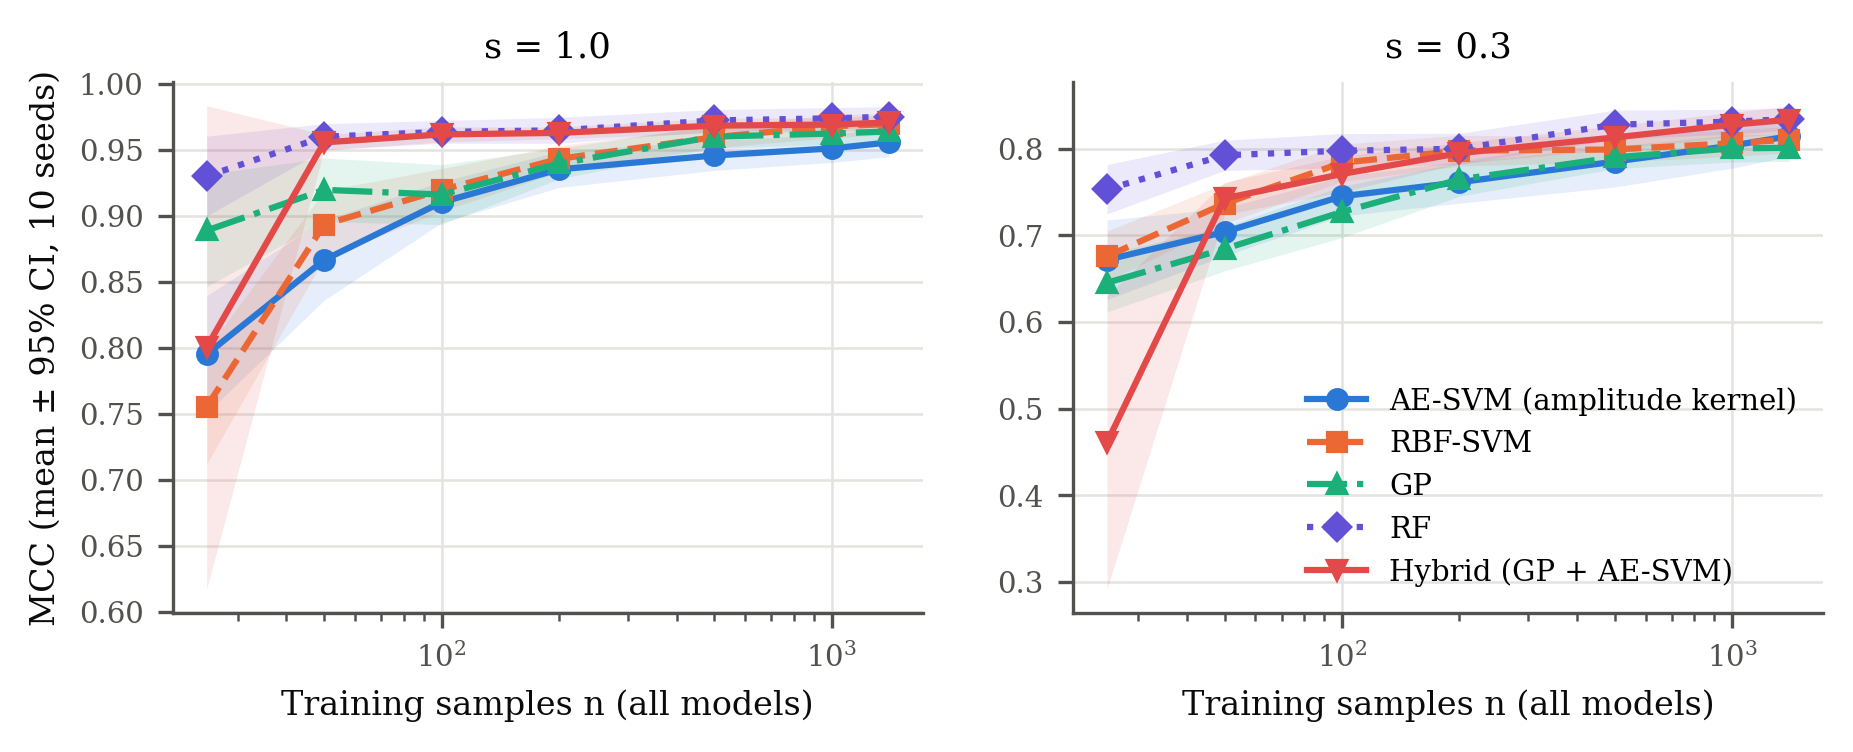
\includegraphics[width=0.8\textwidth]{hyqad/fig3_matched_n.png}\\[2pt]
  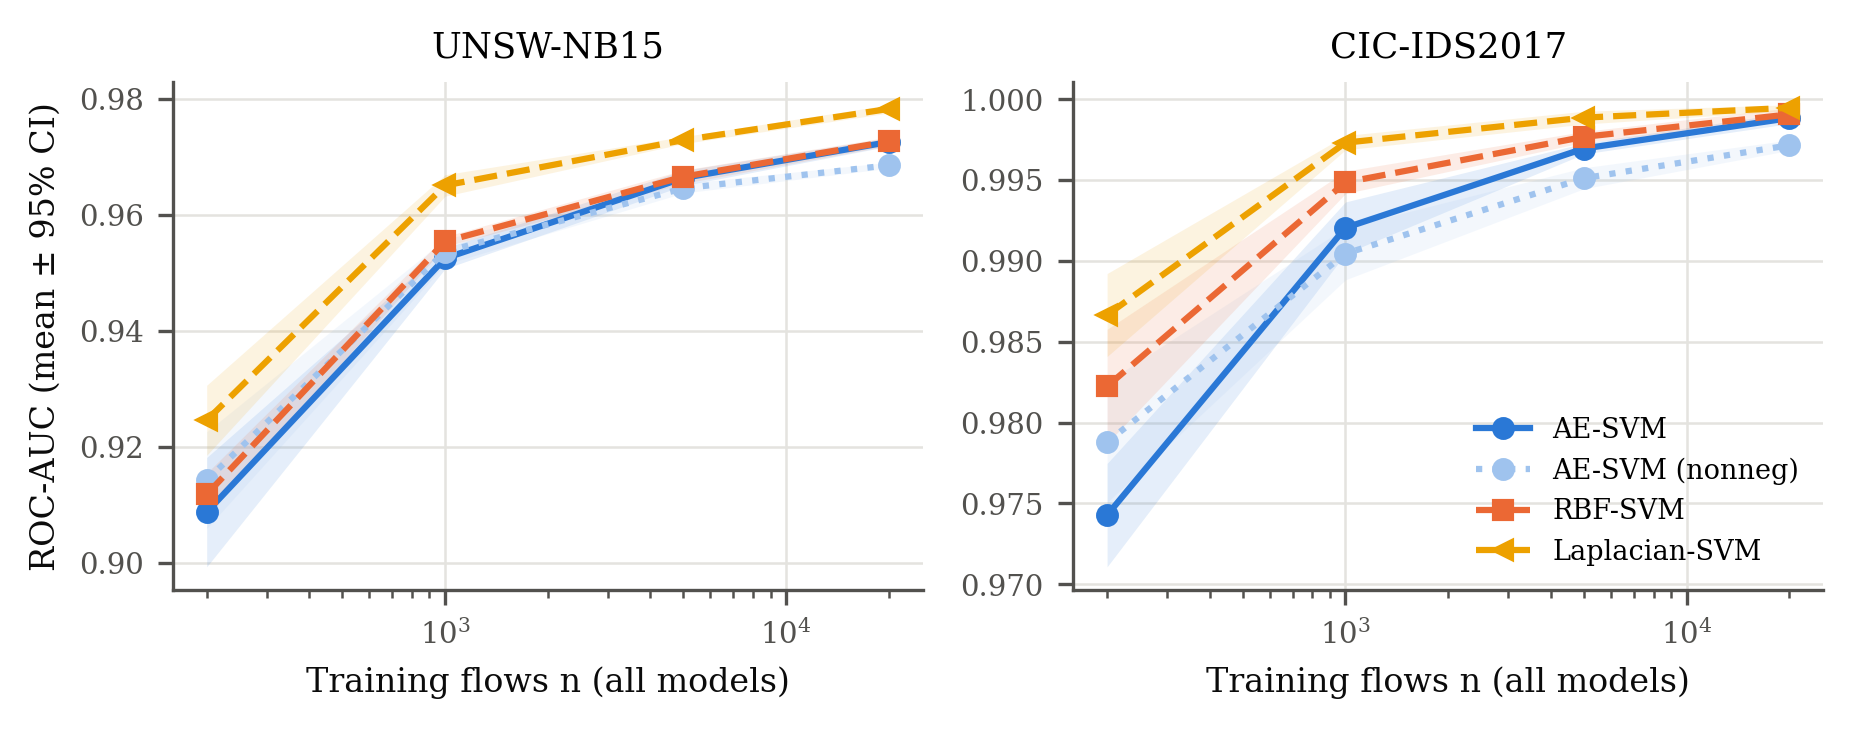
\includegraphics[width=0.8\textwidth]{qztna/fig18_real_matched_n.png}
  \caption{Learning curves with every model trained on the same subsample at each $n$ (mean $\pm$ 95\% CI). Top: QKD telemetry, MCC, at $s=1$ and $s=0.3$. Bottom: public datasets, ROC-AUC.}
  \label{fig:matched}
\end{figure*}

Training every model on the same subsample (Fig.~\ref{fig:matched}) shows no
training size at which the amplitude kernel is reliably ahead. On QKD telemetry
it needs \emph{more} data than RBF to reach the same MCC: at $s=0.3$ it trails
by $0.03$--$0.04$ for $n=50$--$200$ and reaches parity only from $n=1000$. On
synthetic flows it trails by $3.6$ points at $n=50$ and reaches parity by
$n=1000$. @MATCHED_REAL@ Random forests are the most sample-efficient model on
QKD telemetry (MCC $0.75$ at $n=25$, $s=0.3$, against $0.65$--$0.68$ for the
kernels).

\subsection{Generalization to unseen attack types}
\label{sec:res-zeroday}

\begin{figure*}[t]
  \centering
  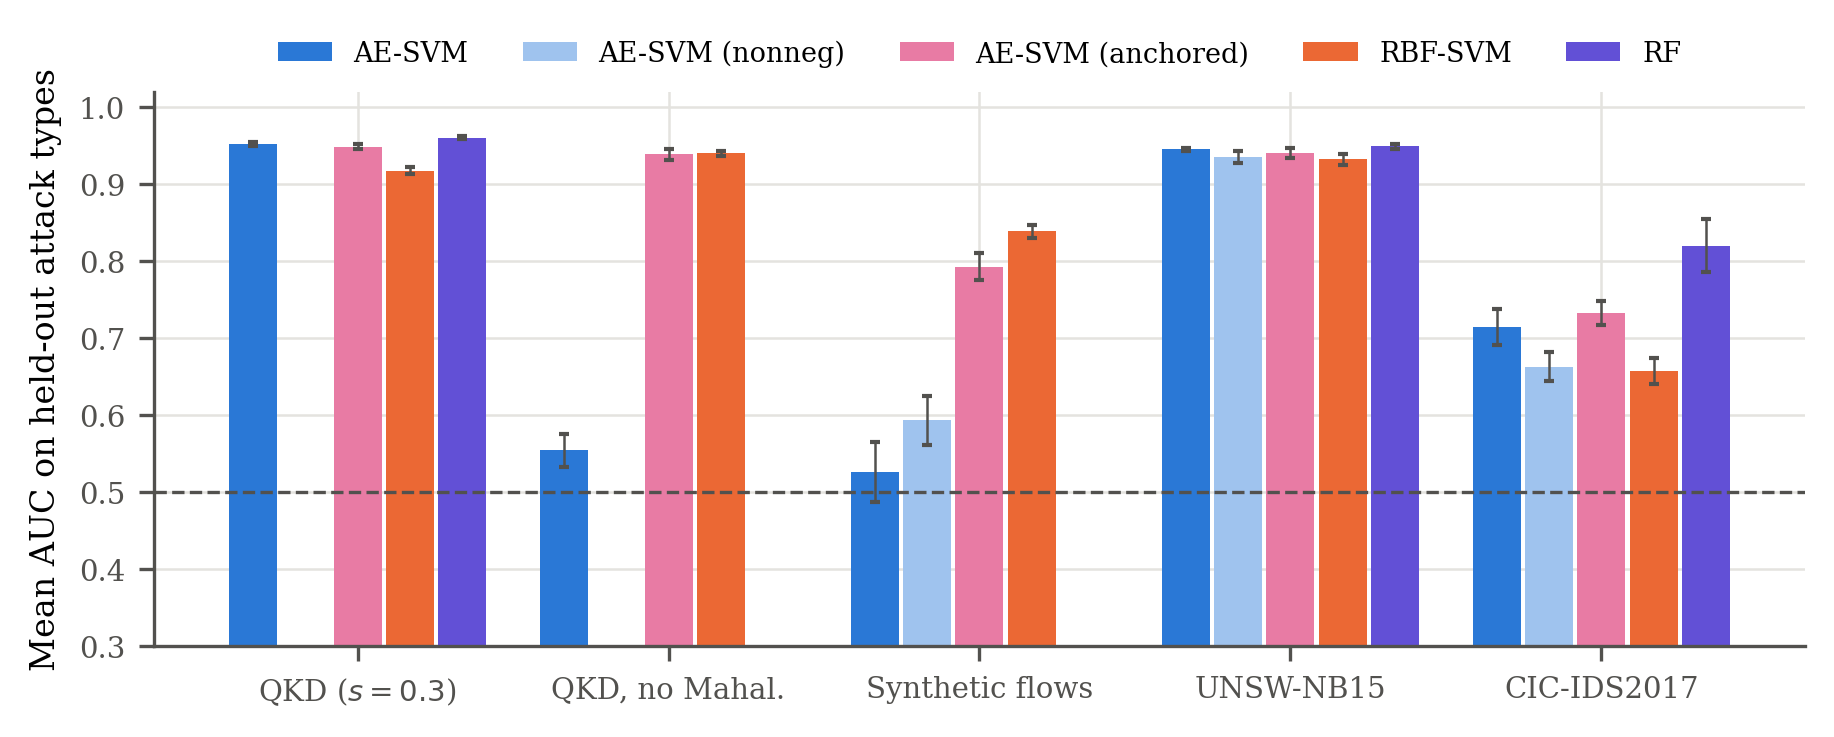
\includegraphics[width=0.9\textwidth]{combined/fig_zeroday_all.png}
  \caption{Mean ROC-AUC on held-out attack types (leave one type or family out; mean $\pm$ 95\% CI over seeds). ``QKD, no Mahal.'' removes the Mahalanobis feature, the only QKD feature that carries the input's magnitude.}
  \label{fig:zeroday}
\end{figure*}

Fig.~\ref{fig:zeroday} shows that unseen-attack behavior differs sharply by
domain. On synthetic flows, plain AE-SVM fails: its mean held-out AUC is $0.526$
against $0.839$ for RBF-SVM, with every held-out type between $0.45$ and $0.61$. On
QKD telemetry it generalizes as well as RF and better than RBF-SVM (mean AUC
$0.952$ vs.\ $0.917$ at $s=0.3$), but only because the feature map contains a
Mahalanobis distance to normal operation, which is a magnitude: removing that one
feature drops AE-SVM to $0.554$ ($0.635$ at $s=1$) while RBF-SVM is unaffected
($0.940$, $0.987$).

The public benchmarks do not show the failure. @ZERODAY_REAL@ On CIC-IDS2017 every
supervised model struggles on some held-out families (Bot, BruteForce,
PortScan), and the benign-only autoencoder, which never sees any attack, is the
most robust detector, as the closed-world critique of supervised intrusion
detection~\cite{sommer2010outside} would predict.

\subsection{Mechanism}
\label{sec:res-mechanism}

Corollary~\ref{cor:inv} offers two explanations for the controlled-setting
failures: sign ambiguity ($\mathbf{x}$ and $-\mathbf{x}$ look identical) and norm
invariance. Interventions separate them. Mapping inputs to $[0,1]^d$ removes the
sign ambiguity but keeps norm invariance; it raises synthetic-flow zero-day AUC
only from $0.526$ to $0.593$. The norm anchor of Eq.~\eqref{eq:anchor} restores the
norm; it raises the same number to $0.793$, and restores QKD zero-day AUC without
the Mahalanobis feature to $0.939$ ($s=0.3$) and $0.980$ ($s=1$), level with
RBF-SVM. @ANCHOR_REAL_ZD@ The constant $c$ is set by the median-norm rule from
training data; a sweep on synthetic flows (two seeds) gives mean zero-day AUC
$0.57$, $0.80$, $0.77$, $0.65$ and $0.53$ for $c=1,4,8,16,32$; the median training
norm is $6.4$, so the rule lands near the best value without looking at held-out
attacks.

Can one tell in advance which regime a dataset is in? We tried the obvious
statistic: for each held-out attack, the AUC of the input norm alone against the
AUC of a direction-only score. Averaged per domain it is highest where AE-SVM
fails (synthetic flows, norm AUC $0.90$ vs.\ direction AUC $0.66$), but across the
28 held-out splits it does not predict the AE-SVM$-$RBF-SVM gap (Spearman
$\rho=-0.09$, $p=0.65$), and it cannot see the QKD ablation, where removing one
coordinate barely changes the norm's separating power yet flips the outcome.
Which features carry magnitude matters more than how much separation the norm
offers overall. We therefore do not have a reliable a-priori test; the
interventions establish the mechanism where the failure occurs, and a direct
leave-one-attack-out evaluation remains necessary.

\begin{figure*}[t]
  \centering
  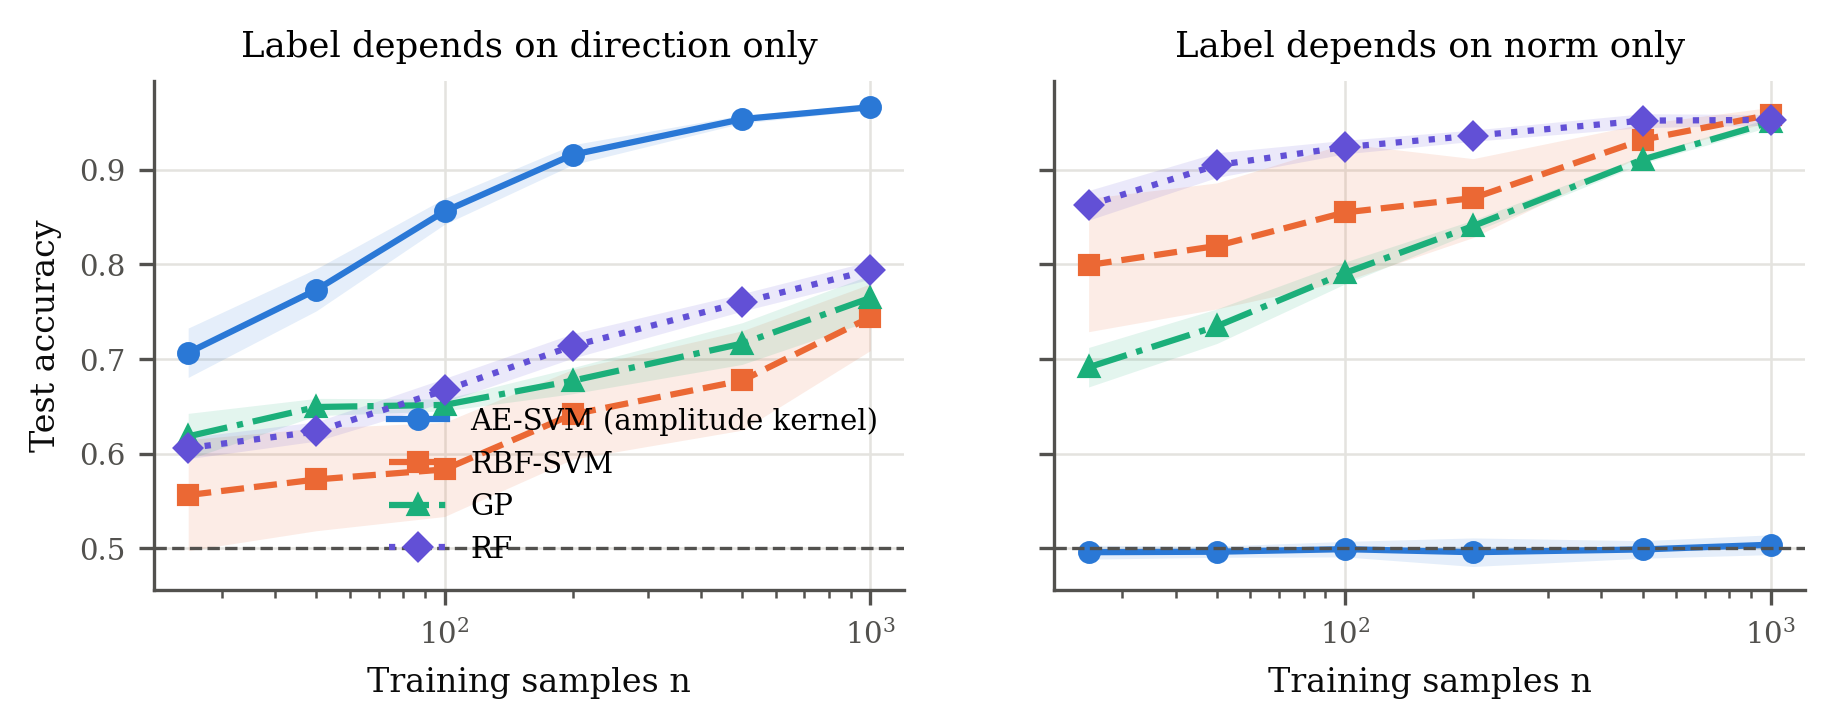
\includegraphics[width=0.64\textwidth]{hyqad/fig8_kernel_crossover.png}\hfill
  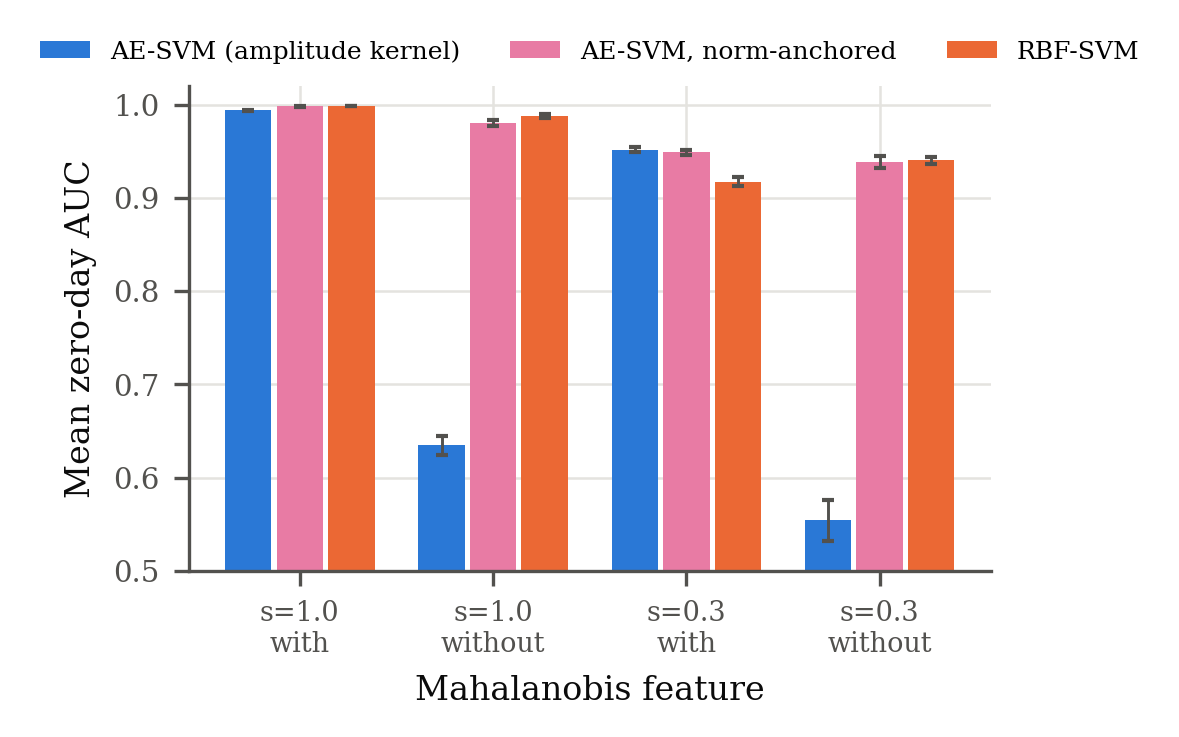
\includegraphics[width=0.34\textwidth]{hyqad/fig9_mahal_ablation.png}
  \caption{Left pair: control tasks in $\mathbb{R}^8$ with heavy-tailed norms; the label depends on direction only or on norm only. Right: QKD zero-day AUC with and without the Mahalanobis feature.}
  \label{fig:mechanism}
\end{figure*}

Two further checks support this account. On control tasks (Fig.~\ref{fig:mechanism},
left) whose label depends only on direction, with a heavy-tailed nuisance norm,
AE-SVM learns from far fewer samples than any baseline ($0.71$ vs.\ $0.56$ for
RBF-SVM at $n=25$; $0.97$ vs.\ $0.74$ at $n=1000$); when the label depends only on
the norm, it is at chance at every $n$. Its inductive bias is therefore real and
predictable; whether it helps on a security dataset depends on how much of the attack signal lies in the norm.
And kernel-target alignment~\cite{cristianini2002kernel} is lower for $K_A$ than for
RBF in every domain and attack type (synthetic flows $0.13$ vs.\ $0.21$; QKD
$0.13$--$0.22$ vs.\ $0.29$--$0.66$@ALIGN_REAL@), so alignment correctly predicts
in-distribution ranking but not, on its own, zero-day behaviour, which depends on
which invariances the kernel imposes.

\subsection{Calibration and selective prediction}
\label{sec:res-calib}

\begin{figure*}[t]
  \centering
  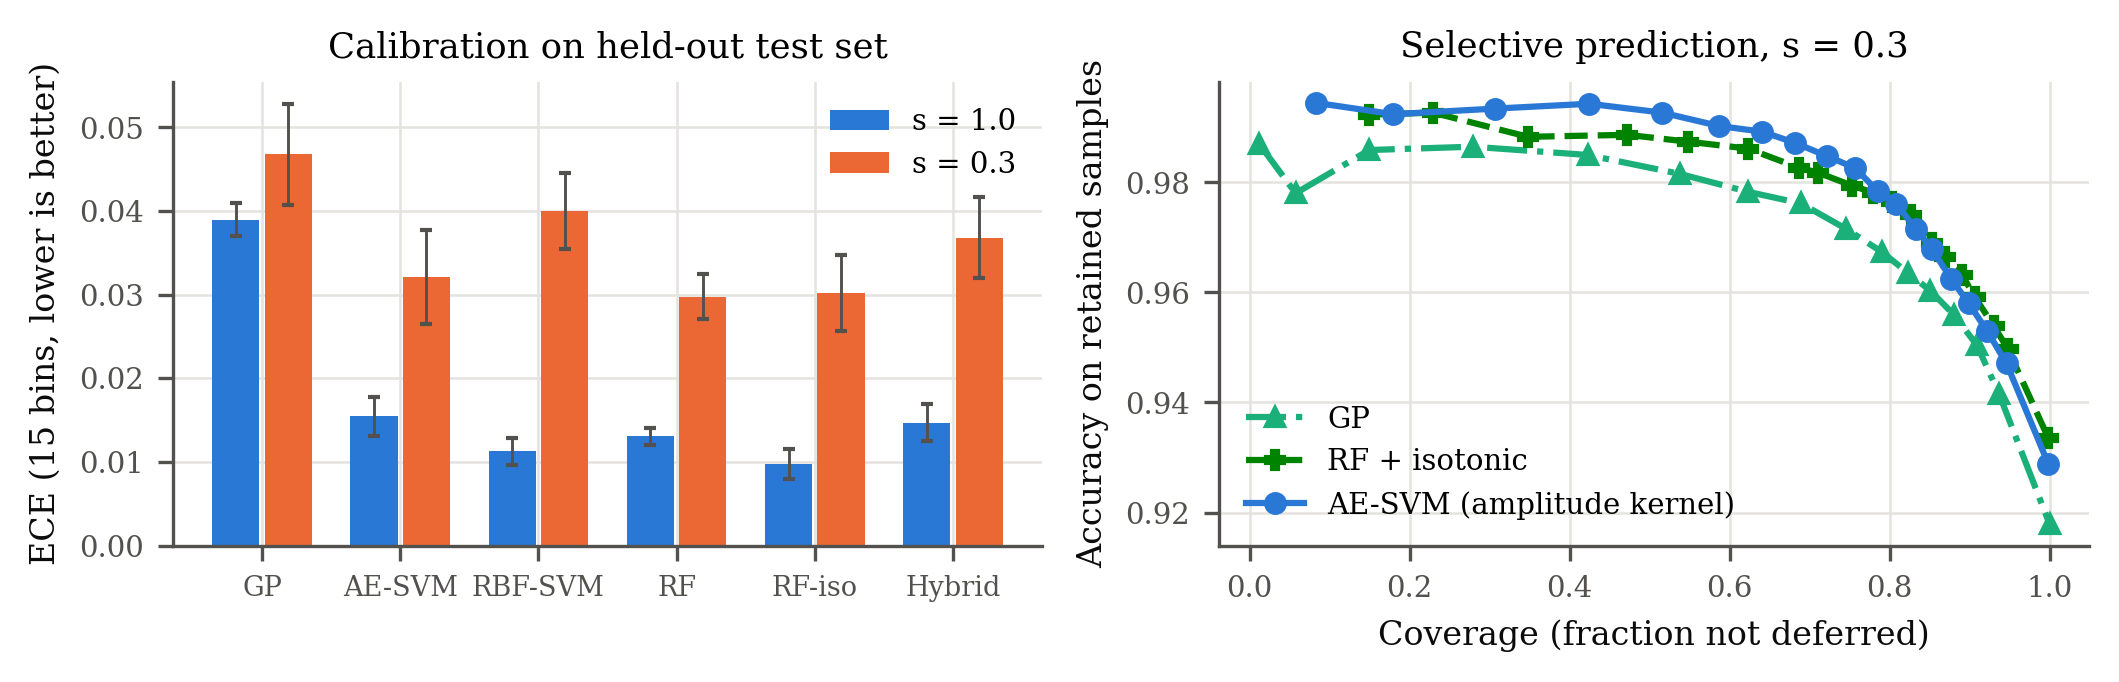
\includegraphics[width=0.8\textwidth]{hyqad/fig6_calibration_selective.png}
  \caption{QKD telemetry. Left: ECE by model. Right: accuracy versus coverage when deferring samples whose uncertainty $u=\sqrt{p(1-p)}$ exceeds a threshold ($s=0.3$).}
  \label{fig:calib}
\end{figure*}

A Gaussian-process posterior is often proposed as the uncertainty signal for
security monitoring. On QKD telemetry the Laplace GP is the least calibrated
supervised model (ECE $0.047\pm0.006$ at $s=0.3$), and isotonic-calibrated RF the
best ($0.030$). For deferral (Fig.~\ref{fig:calib}) the GP's probabilities sit
close to the boundary: at $u<0.3$ it keeps $69\%$ of blocks at $97.6\%$ accuracy,
against $80\%$ for isotonic RF and $79\%$ for AE-SVM at the same accuracy; at
$u<0.1$ it keeps none. The GP's uncertainty also barely rises under a
gradient-free evasion attack ($0.30\to0.33$), so it does not flag evasion either.
Platt-scaled AE-SVM on synthetic flows supports a similar trade-off ($97.4\%$
accuracy at $75.5\%$ coverage).

\subsection{Certified robustness and latency}
\label{sec:res-robust}

Randomized smoothing ($\sigma=0.25$, 300 noise draws, $\alpha=0.05$) gives
comparable certified $\ell_2$ radii for AE-SVM and RBF-SVM on synthetic flows
(mean $0.508$ vs.\ $0.518$; median radius saturated at $0.582$ for both), with
AE-SVM abstaining on $1.8\%$ of points versus none for RBF-SVM. This agrees with
the sensitivity analysis of Section~\ref{sec:kernel}: normalization does not
confer uniform robustness. All detectors are fast. In batch inference AE-SVM
costs $0.008$\,ms per QKD block and $0.0048$\,ms per synthetic flow with $50$
Nystr\"om landmarks, about $1.2\times$ faster than RBF-SVM, because it avoids an
exponential per landmark; tree ensembles and the GP are slower but still far
below any per-flow budget.@LATENCY_REAL@

\section{Discussion}
\label{sec:discussion}

\subsection{What the results say about quantum kernels in security}
Our evidence concerns one encoding, but it is the encoding most often used.
Amplitude encoding brings no in-distribution advantage over an RBF kernel
trained on the same data in any of four datasets, and at small $n$ it needs more
data, not less. Its distinctive property is an invariance, not a capacity: it
sees direction and discards magnitude. That is an advantage when magnitude is a
nuisance, as in our direction-only control task, and a liability when unseen
attacks differ from normal traffic mainly in magnitude, as in both of our
controlled settings. On real traffic, where attack families also differ in
\emph{which} features are active, the liability did not materialize, and the
kernel generalized slightly better than RBF. Two further points. (i) Nothing here
bears on quantum speed-ups: $K_A$ is classically easy, and the slow circuit
simulation that limits some published comparisons to a few dozen samples is an
artifact. (ii) The invariance analysis applies to any fidelity kernel whose
state preparation normalizes its input. A third, methodological point is that
controlled simulators alone would have led us to the wrong general conclusion;
the public benchmarks reversed it.

\subsection{Recommendations}
For practitioners evaluating quantum or quantum-inspired kernels for security
detection we recommend: (1) compare against classical kernels trained on the
\emph{same} data at every $n$; (2) report leave-one-attack-out results on real
traffic, since in-distribution accuracy hid the largest effect in this study and
simulators alone pointed to the wrong general conclusion; (3) check which
input transformations the kernel is invariant to, and whether any feature
re-injects what it discards; (4) if amplitude encoding is used, anchor the norm
(Eq.~\eqref{eq:anchor}), which repaired every failure we observed@ANCHOR_SAFE@; and (5) for simulated telemetry, report single-feature
separability and a signature-strength sweep, because a simulator without
operating drift can make any detector look perfect.

\subsection{Threats to validity}
\textit{Simulation.} QKD results come from a simulator whose attack magnitudes
are modeling assumptions; the strength axis shows how conclusions move with
signature size but does not fix a realistic $s$. Synthetic flows are a
marginal-plus-copula model, not packet-level traffic. The public datasets
mitigate this for network flows but not for QKD, for which no public attack
telemetry exists to our knowledge.
\textit{Datasets.} UNSW-NB15 and CIC-IDS2017 have known labeling and
distribution artifacts; we use the official UNSW-NB15 partition, de-duplicate
CIC-IDS2017, and subsample to 20,000 training flows per seed, which favors kernel
methods relative to full-data tree ensembles.
\textit{Models.} Kernel hyperparameters ($C=1$, median-heuristic bandwidths) were
not tuned per dataset, for any kernel; tuning could change small gaps but is
unlikely to close the $0.3$-AUC zero-day gaps in the controlled settings. Nystr\"om approximation with
$1000$ landmarks may understate exact-kernel accuracy equally for all kernels.
\textit{Zero-day protocol.} Leaving out one attack family is a proxy for novel
attacks; a real novel attack may be closer to, or farther from, the training
families.
\textit{Robustness.} Certified radii are for $\ell_2$ noise on standardized
features and do not cover semantic or adaptive evasion.

\section{Conclusion}
\label{sec:conclusion}

We evaluated the amplitude-encoding quantum kernel---exactly, at every training
size, against classical kernels trained on the same data---on QKD telemetry,
synthetic zero-trust flows, UNSW-NB15 and CIC-IDS2017. It never beats an RBF
kernel in distribution and needs more data at small $n$. On unseen attack types
it fails in both controlled settings, because its fidelity kernel discards input
norm, and a one-coordinate norm anchor repairs that failure; on both public
benchmarks it does not fail, and matches or slightly exceeds RBF. Since a simple
statistic did not predict which case applies, quantum and quantum-inspired
detectors should be judged under a matched-scale protocol that includes
held-out attack families on real traffic, with their invariances analysed
before deployment.

\section*{Code and Data Availability}
All code, the two simulators, dataset preparation scripts for the public
benchmarks, experiment drivers and every result file behind the tables and
figures are available at \url{https://github.com/arnavk23/quasar-security}.

\bibliographystyle{IEEEtran}
\bibliography{../references}

\end{document}
